\documentclass[conference]{IEEEtran}
\IEEEoverridecommandlockouts
% The preceding line is only needed to identify funding in the first footnote. If that is unneeded, please comment it out.
\usepackage{cite}
\usepackage{amsmath,amssymb,amsfonts}
\usepackage{algorithmic}
\usepackage{graphicx}
\usepackage{textcomp}
\usepackage{xcolor}
\def\BibTeX{{\rm B\kern-.05em{\sc i\kern-.025em b}\kern-.08em
    T\kern-.1667em\lower.7ex\hbox{E}\kern-.125emX}}


\def\IEEEkeywordsname{Keywords}

\begin{document}

\title{Differences between Embedded System Operating Systems and Mobile Operating Systems\\
%{\footnotesize \textsuperscript{*}Note: Sub-titles are not captured in Xplore and
%should not be used}
%\thanks{Identify applicable funding agency here. If none, delete this.}
}


\author{\IEEEauthorblockN{Wesly Yii}
\IEEEauthorblockA{\textit{BSc (Hons) in Computer Science} \\
%https://university.sunway.edu.my/tech/bsc-comp-sc
\textit{Sunway University}\\
Selangor, Malaysia\\
18066233@imail.sunway.edu.my}
\and
\IEEEauthorblockN{Tan Chun Ze}
\IEEEauthorblockA{\textit{Bachelor of Software Engineering (Hons)} \\
%https://university.sunway.edu.my/tech/bsc-software-eng
\textit{Sunway University}\\
Selangor, Malaysia\\
15020605@imail.sunway.edu.my}
\and
\IEEEauthorblockN{Lee Ming Zhen}
\IEEEauthorblockA{\textit{Bachelor of Software Engineering (Hons)} \\
\textit{Sunway University}\\
Selangor, Malaysia\\
18088757@imail.sunway.edu.my}
\and
\IEEEauthorblockN{Ryan Aung Yi Yang}
\IEEEauthorblockA{\textit{BSc (Hons) Computer Networking and Security} \\
%https://university.sunway.edu.my/tech/bsc-network-security
%course name too long so truncated some part of it
\textit{Sunway University}\\
Selangor, Malaysia\\
18007906@imail.sunway.edu.my}
}


\maketitle

\begin{abstract}
%This document is a model and instructions for \LaTeX.
%This and the IEEEtran.cls file define the components of your paper [title, text, heads, etc.]. *CRITICAL: Do Not Use Symbols, Special Characters, Footnotes, 
%or Math in Paper Title or Abstract.
\end{abstract}

\begin{IEEEkeywords}
embedded systems, mobile operating systems, operating systems, difference, compare
\end{IEEEkeywords}

\section{Introduction}
%This document is a model and instructions for \LaTeX.
%Please observe the conference page limits. 

\section{Background}
\subsection{Embedded system OS}

\paragraph{What is it about?}\mbox{} \\
Embedded system operating system is a type of operating system that is created to carry out distinct processes for particular devices in order for them to operate optimally. In other words, it is just like having software embedded in a one purpose computer hardware system.They belong to a category of specialized operating systems meaning that they function to perform tasks that are highly specific. Hence, they are more resource efficient than other operating systems but at the same time they are limited in terms of functions. Embedded system operating systems may exist as a standalone independent system or belong as a part of something bigger.There are five types of embedded operating system; Multi-Tasking Operating System, Rate Monotonic Operating System, Preemptive Operating System, Single System Control Loop and Real Time Operating System. Generally, Its main focus is to let a certain device function as intended by running its codes.\\

\\
\paragraph{Why the need for it?}\mbox{} \\
Embedded systems operating systems are everywhere nowadays. It has basically been incorporated in the daily routines of humans and is gradually turning life to be more convenient. There is a need for it as it is able to fill in a niche in our lives. The need for it lies in how embedded operating systems can perform a dedicated function for a specific device to run while also allow it to be less demanding in terms of resource consumption. Devices such as cameras, medical equipment, household appliances all require an embedded operating system to work. Some of it are also designed to be able to withstand harsh temperatures and environments in which other operating systems will fail. Therefore, an embedded operating system is needed to let a single-functioned device to work as intended.

\\
\paragraph{What is the application?}\mbox{} \\
Embedded operating systems are applied in many ways. Applications of it include Embedded Linux, iOS, Windows Mobile Operating System, Blackberry Operating System, and Symbian.A Linux operating system that is utilized within embedded devices and appliances are called Embedded Linux.

\subsection{Mobile OS}\\
\paragraph{What is it about?}\mbox{} \\
A mobile OS, short for mobile operating system, is another type of operating system that is created for the sole purpose of powering mobile devices. These mobile devices include PDAs, tablets, smartphones etc. Similar to how a Windows operating system works in a desktop, a mobile operating system allows different kinds of applications to run on a mobile device by serving as a software platform beneath the apps. All the features and functions that are available on mobile devices are all set by the corresponding mobile operating system.On top of that, mobile operating systems will also be in control of the third-party programs that are used on the mobile device.
\\
\paragraph{Why the need for it?}\mbox{} \\
Technically, smartphones do not require an operating system and the device can just run without problem but it would be a mess since there will be no operating system present to manage the memory, storage and applications. Therefore, a mobile operating system is essential for mobile devices to run ideally. A mobile operating system would enable multitasking, which means that multiple applications can run at one time. It will also allow the users to adjust the brightness and volume of all the applications through a single button. Other than that, applications would then be compatible and portable across multiple devices of different brands.
\\
\paragraph{What is the application?}\mbox{} \\
Some notable examples of mobile operating systems are iOS which powers apple devices and Google’s Android which powers android devices. The differences between iOS and Android is that iOS is designed to only run on Apple devices within its XNU kernel while Android is an open source software which implies that it can be used by other mobile device manufacturers who are then able to customize the Android source code to fit their own device’s needs. Apple has also released other mobile OS meant for their Apple watch and iPad which is watchOS and iPadOS respectively. Other than the two well-known mobile OS, there are also many different mobile OS out there but with lower adoption rates such as the KaiOS and the Sailfish OS. KaiOS is mostly used for dumb phones and has features like Google Assistant while the Sailfish OS is mostly used for Sony mobile devices albeit both run on the Linux kernel. On top of that, there is an up and coming OS which is Huawei’s HarmonyOS that was released in 2019. It aims to power devices in a more efficient way in terms of better memory and storage management by making the codes more streamlined. This newly created OS wants to create one ecosystem for every device to share by using the ‘single kernel across devices approach’.It is also set to be Android’s newest rival as it is also released as an open source platform.



\section{In-depth review and discussion}
There are many types of embedded systems that use different operating systems based on suitability. The most often used embedded system is real-time embedded system (RTOS) according to SILBERSCHATZ.et al [1, p.83] due to the wide range of usage from household appliances to automotive and aerospace systems that requires monitoring real-time events.

QNX is one of the operating systems used in real-time embedded systems. QNX heavily relies on Microkernel architecture to support its own operating system.

\begin{center}
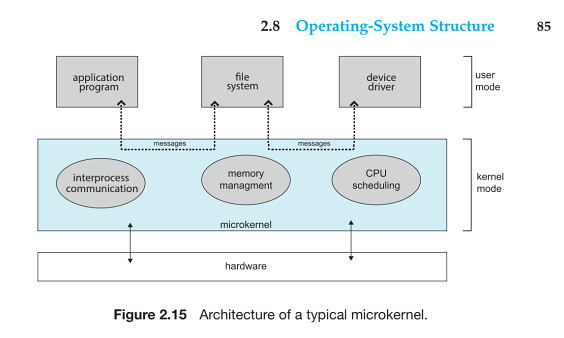
\includegraphics[scale=0.4]{./images/QNX_OS.png}
\end{center}
\subsection{Reason for using Microkernel in QNX}
%\subsection{Efficiency}
\paragraph{Efficiency}\mbox{} \\
Microkernels require less resources to operate as they only contain essential functions(which are interprocess communication, memory management and CPU scheduling) to operate, it allows handling process and memory management to be more efficient. [1] With the benefits of minimal requirement of resources reduce the cost of building embedded systems.
\\
%\subsection{Extentability}
\paragraph{Extentability}\mbox{} \\
%\paragraph{}
Any services can be implemented easily in the user mode without affecting the kernel mode[1]. As a result, any services that need to be updated or modified can be done easily.
\\
%\subsection{Security and Reliability}
\paragraph{Security and reliability}\mbox{} \\
%\paragraph{}
The kernel space will not be affected if any of the services is damaged, because services are only implemented in user mode instead of kernel mode according to SILBERSCHATZ.et al[1]. Damaged kernels can cause serious issues during real-time scenarios. For instance, failure of an anti-lock braking system causing severe accidents that will lead to high chances of deaths. Therefore, security and reliability is crucial to the real-time operating systems.

\subsection{QNX operating system}
\begin{center}
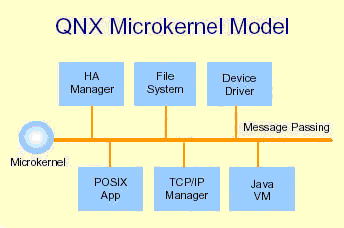
\includegraphics[scale=0.5]{./images/QNX_microkernel_mode.png}
\end{center}
According to https://people.apache.org/~xli/papers/itj2012-mobile-os-trends.pdf, Mobile OS is originally derived from the computer OS which was then evolved into an embedded OS and then to the present smartphone-oriented OS. Throughout the evolutions, the architecture of mobile OS has become simpler compared to the previous versions. In terms of hardware, the factor size of microprocessors and peripherals has been reduced to accommodate the modern design of smartphones. 

%\paragraph{}

\section{Conclusion}

%\section*{Acknowledgment}
%The preferred spelling of the word ``acknowledgment'' in America is without 
%an ``e'' after the ``g''. Avoid the stilted expression ``one of us (R. B. 
%G.) thanks $\ldots$''. Instead, try ``R. B. G. thanks$\ldots$''. Put sponsor 
%acknowledgments in the unnumbered footnote on the first page.

\section*{References}

\end{document}
